% This is samplepaper.tex, a sample chapter demonstrating the
% LLNCS macro package for Springer Computer Science proceedings;
% Version 2.20 of 2017/10/04
%
\documentclass[runningheads]{llncs}
%
\usepackage{graphicx}
% Used for displaying a sample figure. If possible, figure files should
% be included in EPS format.
%\usepackage{tikz}
%\usetikzlibrary{arrows}
\usepackage{verbatim}
\usepackage{algorithm}
\usepackage[noend]{algpseudocode}
\usepackage{amssymb}
\usepackage{amsfonts}
\usepackage{amsmath}
\let\proof\relax\let\endproof\relax
\usepackage{amsthm}
\usepackage{graphicx}
%\usepackage[all]{xy}
\usepackage{array}
\usepackage{enumitem}
%\usepackage{cite}
\usepackage[numbers]{natbib}
\usepackage{wrapfig}
\theoremstyle{definition}
\renewcommand{\qedsymbol}{\hfill\ensuremath{\blacksquare}}
%\newtheorem{definition}{Definition}[section]
% If you use the hyperref package, please uncomment the following line
% to display URLs in blue roman font according to Springer's eBook style:
% \renewcommand\UrlFont{\color{blue}\rmfamily}
\usepackage[breaklinks=true]{hyperref}
\usepackage{breakcites}
\renewcommand\UrlFont{\color{blue}\rmfamily}
\usepackage[colorinlistoftodos,prependcaption,textsize=tiny]{todonotes}

\usepackage{xcolor}
\usepackage{listings}
\definecolor{dkgreen}{rgb}{0,0.6,0}
\definecolor{ltblue}{rgb}{0,0.4,0.4}
\definecolor{dkviolet}{rgb}{0.3,0,0.5}

% lstlisting coq style (inspired from a file of Assia Mahboubi)
\lstdefinelanguage{Coq}{ 
    % Anything betweeen $ becomes LaTeX math mode
    mathescape=true,
    % Comments may or not include Latex commands
    texcl=false, 
    % Vernacular commands
    morekeywords=[1]{Section, Module, End, Require, Import, Export,
        Variable, Variables, Parameter, Parameters, Axiom, Hypothesis,
        Hypotheses, Notation, Local, Tactic, Reserved, Scope, Open, Close,
        Bind, Delimit, Definition, Let, Ltac, Fixpoint, CoFixpoint, Add,
        Morphism, Relation, Implicit, Arguments, Unset, Contextual,
        Strict, Prenex, Implicits, Inductive, CoInductive, Record,
        Structure, Canonical, Coercion, Context, Class, Global, Instance,
        Program, Infix, Theorem, Lemma, Corollary, Proposition, Fact,
        Remark, Example, Proof, Goal, Save, Qed, Defined, Hint, Resolve,
        Rewrite, View, Search, Show, Print, Printing, All, Eval, Check,
        Projections, inside, outside, Def},
    % Gallina
    morekeywords=[2]{forall, exists, exists2, fun, fix, cofix, struct,
        match, with, end, as, in, return, let, if, is, then, else, for, of,
        nosimpl, when},
    % Sorts
    morekeywords=[3]{Type, Prop, Set, true, false, option},
    % Various tactics, some are std Coq subsumed by ssr, for the manual purpose
    morekeywords=[4]{pose, set, move, case, elim, apply, clear, hnf,
        intro, intros, generalize, rename, pattern, after, destruct,
        induction, using, refine, inversion, injection, rewrite, congr,
        unlock, compute, ring, field, fourier, replace, fold, unfold,
        change, cutrewrite, simpl, have, suff, wlog, suffices, without,
        loss, nat_norm, assert, cut, trivial, revert, bool_congr, nat_congr,
        symmetry, transitivity, auto, split, left, right, autorewrite},
    % Terminators
    morekeywords=[5]{by, done, exact, reflexivity, tauto, romega, omega,
        assumption, solve, contradiction, discriminate},
    % Control
    morekeywords=[6]{do, last, first, try, idtac, repeat},
    % Comments delimiters, we do turn this off for the manual
    morecomment=[s]{(*}{*)},
    % Spaces are not displayed as a special character
    showstringspaces=false,
    % String delimiters
    morestring=[b]",
    morestring=[d],
    % Size of tabulations
    tabsize=3,
    % Enables ASCII chars 128 to 255
    extendedchars=false,
    % Case sensitivity
    sensitive=true,
    % Automatic breaking of long lines
    breaklines=false,
    % Default style fors listings
    basicstyle=\small,
    % Position of captions is bottom
    captionpos=b,
    % flexible columns
    columns=[l]flexible,
    % Style for (listings') identifiers
    identifierstyle={\ttfamily\color{black}},
    % Style for declaration keywords
    keywordstyle=[1]{\ttfamily\color{dkviolet}},
    % Style for gallina keywords
    keywordstyle=[2]{\ttfamily\color{dkgreen}},
    % Style for sorts keywords
    keywordstyle=[3]{\ttfamily\color{ltblue}},
    % Style for tactics keywords
    keywordstyle=[4]{\ttfamily\color{dkblue}},
    % Style for terminators keywords
    keywordstyle=[5]{\ttfamily\color{dkred}},
    %Style for iterators
    %keywordstyle=[6]{\ttfamily\color{dkpink}},
    % Style for strings
    stringstyle=\ttfamily,
    % Style for comments
    commentstyle={\ttfamily\color{dkgreen}},
    %moredelim=**[is][\ttfamily\color{red}]{/&}{&/},
    literate=
    {\\forall}{{\color{dkgreen}{$\forall\;$}}}1
    {\\exists}{{$\exists\;$}}1
    {<-}{{$\leftarrow\;$}}1
    {=>}{{$\Rightarrow\;$}}1
    {==}{{\code{==}\;}}1
    {==>}{{\code{==>}\;}}1
    %    {:>}{{\code{:>}\;}}1
    {->}{{$\rightarrow\;$}}1
    {<->}{{$\leftrightarrow\;$}}1
    {<==}{{$\leq\;$}}1
    {\#}{{$^\star$}}1 
    {\\o}{{$\circ\;$}}1 
    {\@}{{$\cdot$}}1 
    {\/\\}{{$\wedge\;$}}1
    {\\\/}{{$\vee\;$}}1
    {++}{{\code{++}}}1
    {~}{{\ }}1
    {\@\@}{{$@$}}1
    {\\mapsto}{{$\mapsto\;$}}1
    {\\hline}{{\rule{\linewidth}{0.5pt}}}1
    %
  }[keywords,comments,strings]
  

\usepackage{tikz}
\usetikzlibrary{arrows}
\usepackage{multirow,tabularx}
\usepackage{amssymb}
\usepackage{amsmath}
\usepackage[numbers]{natbib}
\usepackage{array}
\usepackage{subfig}
\usepackage{tcolorbox}

\begin{document}
%
\title{Ideas Surrounding Protocol Orderings \thanks{Supported by organization x.}}
%
%\titlerunning{Abbreviated paper title}
% If the paper title is too long for the running head, you can set
% an abbreviated paper title here
%
\author{Anna Fritz}
%
\authorrunning{A. Fritz}
% First names are abbreviated in the running head.
% If there are more than two authors, 'et al.' is used.
%
\institute{Institute for Information Sciences \\ The
  University of Kansas \\ Lawrence, KS 66045 \\
  \email{\{authors\}@ku.edu}}
%
\maketitle              % typeset the header of the contribution
%
\begin{abstract}
The abstract should briefly summarize the contents of the paper in
15--250 words.

\keywords{First keyword  \and Second keyword \and Another keyword.}
\end{abstract}
%
%
\section{Goals}

In this work we aim to introduce a means to produce some protocol ordering. When comparing two protocols, say a and b, we hope to be able to say 

\begin{enumerate}
    \item a $\leq$ b \& a $\neq$ b $\implies$ a $<$ b
    \item a $\leq$ b \& a $=$ b $\implies$ a $=$ b
    \item a \& b are incomparable  
\end{enumerate}
\section{Necessary Background}

\begin{definition}[Homomorphism]
    A (graph) homomorphism $\eta : G \to H$ between graphs $G = (N_G, E_G, l_G)$ and $H = (N_H, E_H, l_H)$ is a function $\eta : N_G \to N_H$ on the nodes such that for every edge $(n_1, n_2) \in E_G$, $(\eta(n_1), \eta(n_2)) \in E_H$, and for every node $n \in N_G$, $l_G(n) = l_H(n)$.  \cite{Rowe:2021:OnOrdering}
\end{definition}

\begin{definition}[Supports/Covers]
    Given two sets of graphs S and T, we say that S supports T iff for every $H \in T$, there is some $G \in S$, such that $G \leq H$. We  say that T covers S iff for every $G \in S$ there is some $H \in T$ such that $G \leq H. $\cite{Rowe:2021:OnOrdering}
\end{definition}



%\begin{theorem}[Theorem]
    % This is a sample theorem. 
%\end{theorem}
    %
    % the environments 'definition', 'lemma', 'proposition', 'corollary',
    % 'remark', and 'example' are defined in the LLNCS documentclass as well.
    %
% \begin{proof}
% Proofs, examples, and remarks have the initial word in italics,
% while the following text appears in normal font.
% \end{proof}

\section{Examples}
\newcolumntype{M}[1]{>{\centering\arraybackslash}m{#1}}
\newcolumntype{N}{@{}m{0pt}@{}}

We motivate this work specifically in the context of attack trees. 

\subsection{Chase Model Finder}

\begin{center}
    \begin{tabular}{ M{2.75cm} | c }
     Protocol Name & Actual protocol  \\
     \hline 
     \hline    
     sys & *target: @p4 (vc p4 sys)  \\ 
     \hline
     vc sys seq & *target: @p3 [(a1 p4 vc) $+<+$ @p4 (vc p4 sys)]   \\
     \hline   
     ker vc sys seq & *target: @p4 [(ker p4 vc) $+<+$ @p4 (vc p4 sys)] \\ 
     \hline 
     rtm ker vc sys seq & *target: @p1 [(rtm p4 ker) $+<+$ @p4 [(ker p4 vc) $+<+$ @p4 (vc p4 sys)]] 
    \end{tabular}
    \end{center}


%\begin{figure}[htpb]
%    \centering 
%    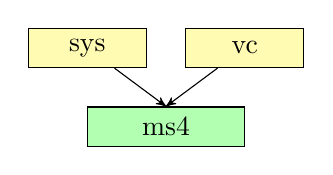
\begin{tikzpicture}[->,>=stealth']

    \node[rectangle,
          draw,
          fill = green!30,
          minimum width = 2cm, 
          minimum height = 0.5cm
          ] (ms4) at (0,0) {};
    \node[] at (ms4.center) {ms4};


    \node[rectangle,
        draw,
        fill = yellow!30,
        minimum width = 1.5cm, 
        minimum height = 0.5cm
        ] (sys) at (-1,1) {};
    \node[] at (sys.center) {sys};

    \node[rectangle,
        draw,
        fill = yellow!30,
        minimum width = 1.5cm, 
        minimum height = 0.5cm
        ] (vc) at (1,1) {};
    \node[] at (vc.center) {vc};


    \path[every node/.style={font=\sffamily\small}]
    %host1 path
    (vc) edge [] node [right] {} (ms4.north) 
    (sys) edge [] node [right] {} (ms4.north) ;


\end{tikzpicture}
%    \label{fig:sys1}
%\end{figure}

\begin{figure}
\begin{center}
    \begin{tabular}{ M{3.75cm} | M{5cm} }
            sys & vc sys seq  \\
            \hline
            \hline
            \\ 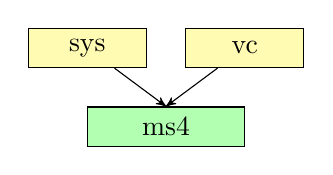
\begin{tikzpicture}[->,>=stealth']

    \node[rectangle,
          draw,
          fill = green!30,
          minimum width = 2cm, 
          minimum height = 0.5cm
          ] (ms4) at (0,0) {};
    \node[] at (ms4.center) {ms4};


    \node[rectangle,
        draw,
        fill = yellow!30,
        minimum width = 1.5cm, 
        minimum height = 0.5cm
        ] (sys) at (-1,1) {};
    \node[] at (sys.center) {sys};

    \node[rectangle,
        draw,
        fill = yellow!30,
        minimum width = 1.5cm, 
        minimum height = 0.5cm
        ] (vc) at (1,1) {};
    \node[] at (vc.center) {vc};


    \path[every node/.style={font=\sffamily\small}]
    %host1 path
    (vc) edge [] node [right] {} (ms4.north) 
    (sys) edge [] node [right] {} (ms4.north) ;


\end{tikzpicture} & 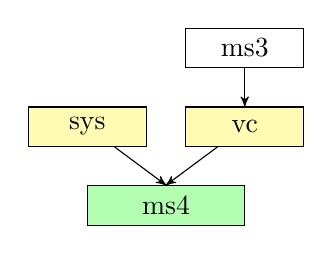
\begin{tikzpicture}[->,>=stealth']

    \node[rectangle,
          draw,
          fill = green!30,
          minimum width = 2cm, 
          minimum height = 0.5cm
          ] (ms4) at (0,0) {};
    \node[] at (ms4.center) {ms4};


    \node[rectangle,
        draw,
        fill = yellow!30,
        minimum width = 1.5cm, 
        minimum height = 0.5cm
        ] (sys) at (-1,1) {};
    \node[] at (sys.center) {sys};

    \node[rectangle,
        draw,
        fill = yellow!30,
        minimum width = 1.5cm, 
        minimum height = 0.5cm
        ] (vc) at (1,1) {};
    \node[] at (vc.center) {vc};

    \node[rectangle,
        draw,
        minimum width = 1.5cm, 
        minimum height = 0.5cm
        ] (ms3) at (1,2) {};
    \node[] at (ms3.center) {ms3};


    \path[every node/.style={font=\sffamily\small}]
    %host1 path
    (ms3) edge [] node [right] {} (vc.north)
    (vc) edge [] node [right] {} (ms4.north) 
    (sys) edge [] node [right] {} (ms4.north) ;


\end{tikzpicture}  \\ [50pt]
            \\ \begin{tikzpicture}[->,>=stealth']

    \node[rectangle,
          draw,
          fill = green!30,
          minimum width = 2cm, 
          minimum height = 0.5cm
          ] (ms4) at (0,0) {};
    \node[] at (ms4.center) {ms4};


    \node[rectangle,
        draw,
        fill = yellow!30,
        minimum width = 1.5cm, 
        minimum height = 0.5cm
        ] (sys) at (-1,1) {};
    \node[] at (sys.center) {sys};

    \node[rectangle,
        draw,
        fill = yellow!30,
        minimum width = 1.5cm, 
        minimum height = 0.5cm
        ] (ker) at (1,1) {};
    \node[] at (ker.center) {ker};


    \path[every node/.style={font=\sffamily\small}]
    %host1 path
    (vc) edge [] node [right] {} (ms4.north) 
    (sys) edge [] node [right] {} (ms4.north) ;


\end{tikzpicture} & 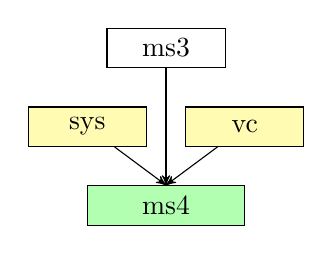
\begin{tikzpicture}[->,>=stealth']

    \node[rectangle,
          draw,
          fill = green!30,
          minimum width = 2cm, 
          minimum height = 0.5cm
          ] (ms4) at (0,0) {};
    \node[] at (ms4.center) {ms4};


    \node[rectangle,
        draw,
        fill = yellow!30,
        minimum width = 1.5cm, 
        minimum height = 0.5cm
        ] (sys) at (-1,1) {};
    \node[] at (sys.center) {sys};

    \node[rectangle,
        draw,
        fill = yellow!30,
        minimum width = 1.5cm, 
        minimum height = 0.5cm
        ] (vc) at (1,1) {};
    \node[] at (vc.center) {vc};

    \node[rectangle,
        draw,
        minimum width = 1.5cm, 
        minimum height = 0.5cm
        ] (ms3) at (0,2) {};
    \node[] at (ms3.center) {ms3};


    \path[every node/.style={font=\sffamily\small}]
    %host1 path
    (ms3) edge [] node [right] {} (ms4.north)
    (vc) edge [] node [right] {} (ms4.north) 
    (sys) edge [] node [right] {} (ms4.north) ;


\end{tikzpicture}  \\ [50pt]  
             & 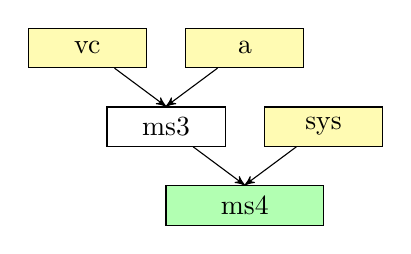
\begin{tikzpicture}[->,>=stealth']

    \node[rectangle,
          draw,
          fill = green!30,
          minimum width = 2cm, 
          minimum height = 0.5cm
          ] (ms4) at (0,0) {};
    \node[] at (ms4.center) {ms4};


    \node[rectangle,
        draw,
        minimum width = 1.5cm, 
        minimum height = 0.5cm
        ] (ms3) at (-1,1) {};
    \node[] at (ms3.center) {ms3};

    \node[rectangle,
        draw,
        fill = yellow!30,
        minimum width = 1.5cm, 
        minimum height = 0.5cm
        ] (sys) at (1,1) {};
    \node[] at (sys.center) {sys};

    \node[rectangle,
        draw,
        fill = yellow!30,
        minimum width = 1.5cm, 
        minimum height = 0.5cm
        ] (vc) at (-2,2) {};
    \node[] at (vc.center) {vc};

    \node[rectangle,
        draw,
        fill = yellow!30,
        minimum width = 1.5cm, 
        minimum height = 0.5cm
        ] (a) at (0,2) {};
    \node[] at (a.center) {a};


    \path[every node/.style={font=\sffamily\small}]
    %host1 path
    (a) edge [] node [right] {} (ms3.north)
    (vc) edge [] node [right] {} (ms3.north)
    (sys) edge [] node [right] {} (ms4.north) 
    (ms3) edge [] node [right] {} (ms4.north) ;


\end{tikzpicture}  \\ [50pt]  
            \\  & 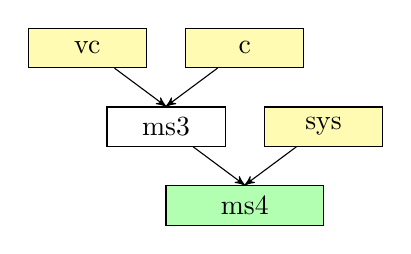
\begin{tikzpicture}[->,>=stealth']

    \node[rectangle,
          draw,
          fill = green!30,
          minimum width = 2cm, 
          minimum height = 0.5cm
          ] (ms4) at (0,0) {};
    \node[] at (ms4.center) {ms4};


    \node[rectangle,
        draw,
        minimum width = 1.5cm, 
        minimum height = 0.5cm
        ] (ms3) at (-1,1) {};
    \node[] at (ms3.center) {ms3};

    \node[rectangle,
        draw,
        fill = yellow!30,
        minimum width = 1.5cm, 
        minimum height = 0.5cm
        ] (sys) at (1,1) {};
    \node[] at (sys.center) {sys};

    \node[rectangle,
        draw,
        fill = yellow!30,
        minimum width = 1.5cm, 
        minimum height = 0.5cm
        ] (vc) at (-2,2) {};
    \node[] at (vc.center) {vc};

    \node[rectangle,
        draw,
        fill = yellow!30,
        minimum width = 1.5cm, 
        minimum height = 0.5cm
        ] (a) at (0,2) {};
    \node[] at (a.center) {c};


    \path[every node/.style={font=\sffamily\small}]
    %host1 path
    (a) edge [] node [right] {} (ms3.north)
    (vc) edge [] node [right] {} (ms3.north)
    (sys) edge [] node [right] {} (ms4.north) 
    (ms3) edge [] node [right] {} (ms4.north) ;


\end{tikzpicture}  \\ [50pt] 
        \end{tabular}
    \end{center}
    \caption{All attack graphs for two protocols}
\end{figure}

We hypothesize that measuring more system components is better. Therefore, we wish to say vc sys seq supports sys. 

\begin{figure}
    \begin{center}
        \begin{tabular}{ M{3.75cm} | M{4.75cm} | M{3.75cm} }
                sys & vc sys seq & ker vc sys seq \\
                \hline
                \hline
                \\ 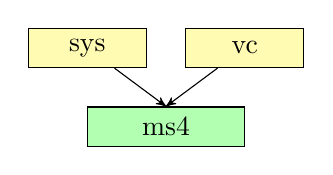
\begin{tikzpicture}[->,>=stealth']

    \node[rectangle,
          draw,
          fill = green!30,
          minimum width = 2cm, 
          minimum height = 0.5cm
          ] (ms4) at (0,0) {};
    \node[] at (ms4.center) {ms4};


    \node[rectangle,
        draw,
        fill = yellow!30,
        minimum width = 1.5cm, 
        minimum height = 0.5cm
        ] (sys) at (-1,1) {};
    \node[] at (sys.center) {sys};

    \node[rectangle,
        draw,
        fill = yellow!30,
        minimum width = 1.5cm, 
        minimum height = 0.5cm
        ] (vc) at (1,1) {};
    \node[] at (vc.center) {vc};


    \path[every node/.style={font=\sffamily\small}]
    %host1 path
    (vc) edge [] node [right] {} (ms4.north) 
    (sys) edge [] node [right] {} (ms4.north) ;


\end{tikzpicture} & 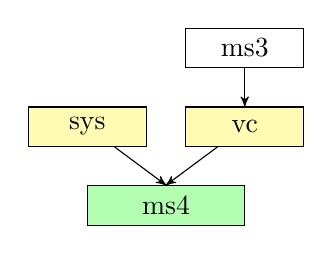
\begin{tikzpicture}[->,>=stealth']

    \node[rectangle,
          draw,
          fill = green!30,
          minimum width = 2cm, 
          minimum height = 0.5cm
          ] (ms4) at (0,0) {};
    \node[] at (ms4.center) {ms4};


    \node[rectangle,
        draw,
        fill = yellow!30,
        minimum width = 1.5cm, 
        minimum height = 0.5cm
        ] (sys) at (-1,1) {};
    \node[] at (sys.center) {sys};

    \node[rectangle,
        draw,
        fill = yellow!30,
        minimum width = 1.5cm, 
        minimum height = 0.5cm
        ] (vc) at (1,1) {};
    \node[] at (vc.center) {vc};

    \node[rectangle,
        draw,
        minimum width = 1.5cm, 
        minimum height = 0.5cm
        ] (ms3) at (1,2) {};
    \node[] at (ms3.center) {ms3};


    \path[every node/.style={font=\sffamily\small}]
    %host1 path
    (ms3) edge [] node [right] {} (vc.north)
    (vc) edge [] node [right] {} (ms4.north) 
    (sys) edge [] node [right] {} (ms4.north) ;


\end{tikzpicture} & cell3 \\ [50pt]
                \\ \begin{tikzpicture}[->,>=stealth']

    \node[rectangle,
          draw,
          fill = green!30,
          minimum width = 2cm, 
          minimum height = 0.5cm
          ] (ms4) at (0,0) {};
    \node[] at (ms4.center) {ms4};


    \node[rectangle,
        draw,
        fill = yellow!30,
        minimum width = 1.5cm, 
        minimum height = 0.5cm
        ] (sys) at (-1,1) {};
    \node[] at (sys.center) {sys};

    \node[rectangle,
        draw,
        fill = yellow!30,
        minimum width = 1.5cm, 
        minimum height = 0.5cm
        ] (ker) at (1,1) {};
    \node[] at (ker.center) {ker};


    \path[every node/.style={font=\sffamily\small}]
    %host1 path
    (vc) edge [] node [right] {} (ms4.north) 
    (sys) edge [] node [right] {} (ms4.north) ;


\end{tikzpicture} & 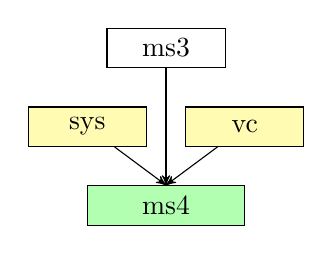
\begin{tikzpicture}[->,>=stealth']

    \node[rectangle,
          draw,
          fill = green!30,
          minimum width = 2cm, 
          minimum height = 0.5cm
          ] (ms4) at (0,0) {};
    \node[] at (ms4.center) {ms4};


    \node[rectangle,
        draw,
        fill = yellow!30,
        minimum width = 1.5cm, 
        minimum height = 0.5cm
        ] (sys) at (-1,1) {};
    \node[] at (sys.center) {sys};

    \node[rectangle,
        draw,
        fill = yellow!30,
        minimum width = 1.5cm, 
        minimum height = 0.5cm
        ] (vc) at (1,1) {};
    \node[] at (vc.center) {vc};

    \node[rectangle,
        draw,
        minimum width = 1.5cm, 
        minimum height = 0.5cm
        ] (ms3) at (0,2) {};
    \node[] at (ms3.center) {ms3};


    \path[every node/.style={font=\sffamily\small}]
    %host1 path
    (ms3) edge [] node [right] {} (ms4.north)
    (vc) edge [] node [right] {} (ms4.north) 
    (sys) edge [] node [right] {} (ms4.north) ;


\end{tikzpicture} & cell6 \\ [50pt]  
                 & 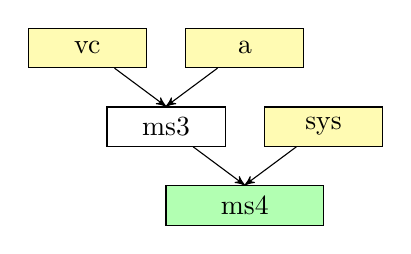
\begin{tikzpicture}[->,>=stealth']

    \node[rectangle,
          draw,
          fill = green!30,
          minimum width = 2cm, 
          minimum height = 0.5cm
          ] (ms4) at (0,0) {};
    \node[] at (ms4.center) {ms4};


    \node[rectangle,
        draw,
        minimum width = 1.5cm, 
        minimum height = 0.5cm
        ] (ms3) at (-1,1) {};
    \node[] at (ms3.center) {ms3};

    \node[rectangle,
        draw,
        fill = yellow!30,
        minimum width = 1.5cm, 
        minimum height = 0.5cm
        ] (sys) at (1,1) {};
    \node[] at (sys.center) {sys};

    \node[rectangle,
        draw,
        fill = yellow!30,
        minimum width = 1.5cm, 
        minimum height = 0.5cm
        ] (vc) at (-2,2) {};
    \node[] at (vc.center) {vc};

    \node[rectangle,
        draw,
        fill = yellow!30,
        minimum width = 1.5cm, 
        minimum height = 0.5cm
        ] (a) at (0,2) {};
    \node[] at (a.center) {a};


    \path[every node/.style={font=\sffamily\small}]
    %host1 path
    (a) edge [] node [right] {} (ms3.north)
    (vc) edge [] node [right] {} (ms3.north)
    (sys) edge [] node [right] {} (ms4.north) 
    (ms3) edge [] node [right] {} (ms4.north) ;


\end{tikzpicture} & cell9 \\ [50pt]  
                \\  & 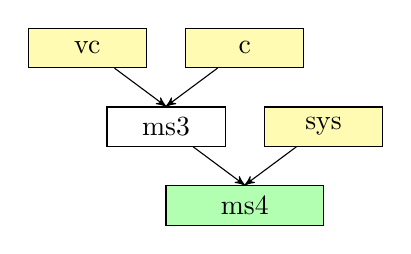
\begin{tikzpicture}[->,>=stealth']

    \node[rectangle,
          draw,
          fill = green!30,
          minimum width = 2cm, 
          minimum height = 0.5cm
          ] (ms4) at (0,0) {};
    \node[] at (ms4.center) {ms4};


    \node[rectangle,
        draw,
        minimum width = 1.5cm, 
        minimum height = 0.5cm
        ] (ms3) at (-1,1) {};
    \node[] at (ms3.center) {ms3};

    \node[rectangle,
        draw,
        fill = yellow!30,
        minimum width = 1.5cm, 
        minimum height = 0.5cm
        ] (sys) at (1,1) {};
    \node[] at (sys.center) {sys};

    \node[rectangle,
        draw,
        fill = yellow!30,
        minimum width = 1.5cm, 
        minimum height = 0.5cm
        ] (vc) at (-2,2) {};
    \node[] at (vc.center) {vc};

    \node[rectangle,
        draw,
        fill = yellow!30,
        minimum width = 1.5cm, 
        minimum height = 0.5cm
        ] (a) at (0,2) {};
    \node[] at (a.center) {c};


    \path[every node/.style={font=\sffamily\small}]
    %host1 path
    (a) edge [] node [right] {} (ms3.north)
    (vc) edge [] node [right] {} (ms3.north)
    (sys) edge [] node [right] {} (ms4.north) 
    (ms3) edge [] node [right] {} (ms4.north) ;


\end{tikzpicture} & cell6 \\ [50pt] 
            \end{tabular}
        \end{center}
        \caption{All attack graphs for two protocols}
    \end{figure}

%
% 
% ---- Bibliography ----
%
% BibTeX users should specify bibliography style 'splncs04'.
% References will then be sorted and formatted in the correct style.
%
%\bibliographystyle{splncs04}
\bibliographystyle{splncsnat}
%\bibliography{sldg}
\bibliography{works}
%
\end{document}
